% !TeX root = ../main.tex

\chapter{网页端动态图生成管理系统}
\label{cha:chapter04}

在第\ref{cha:chapter03}章中,动态图生成工具中的动态图配置使用了JSON格式,用户手动编写与修改较为困难。本章使用网页配置的形式对配置过程进行优化,可以让用户更方便地进行配置与修改。在此基础上,本章中设计并构建了一个完整的网页端动态图生成管理系统,使用Vue.js进行前端整个体系的搭建,其中用ElementUI进行美化,用Echarts进行相关可视化的操作;并且使用Django进行后端Restful API的搭建,将第\ref{cha:chapter03}章中实现的可配置动态图生成工具作为其中的一个组件接入其中,以便用户方便、直观地进行系统的使用。

\section{系统架构}

\begin{figure}
  \centering
  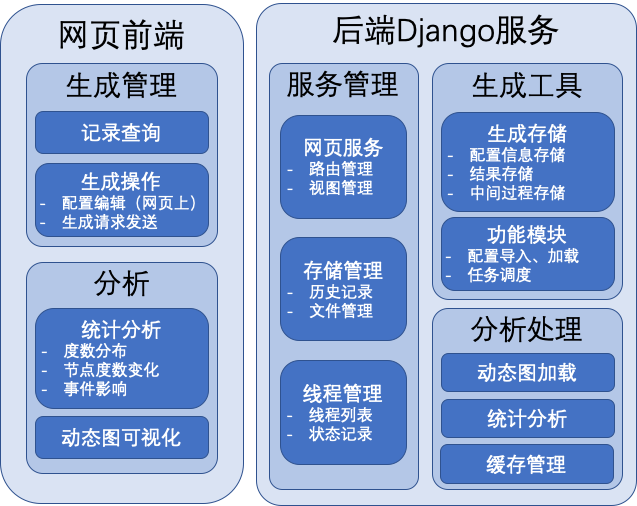
\includegraphics[scale=0.6]{web_system.png}
  \caption{网页端动态图生成管理系统整体架构}
  \label{fig:web_system}
\end{figure}

如图\ref{fig:web_system}所示,系统使用前后端分离的Restful架构设计,在后端Django服务中嵌入第\ref{cha:chapter03}章中实现的可配置动态图生成工具,便于进行处理。

前端部分主要的工作集中于图的配置、生成与后续的分析、可视化操作。其中图的生成命令、生成结果与历史记录、分析数据的获取都用网络请求API与后端进行交互。

后端部分相对较为复杂,关键点在于将生成工具与网页服务结合在一起。

由于生成过程时间较长会阻塞网页请求,因此在系统中使用了多线程的方法,配置了一个专门的线程管理器,每次有生成请求时便分配给一个新的线程,结果查询时会检测线程是否成功结束。这样的设计也可以很好地避免生成工具部分出现问题导致进程挂起,提高了整个系统的可靠性。

由于需要进行大量的生成与结果查询的工作,在后端服务中设计实现了用于结果存储的模块。使用数据库进行配置信息、生成记录、文件存放位置、线程状态等内容的存储。

对于前端的统计分析、可视化需求,为了节省带宽、加快访问速度,避免不必要的前端计算,采用了带有缓存的动态图后端分析处理体系,在后端完成节点度数统计后直接将结果返回,缓存机制可以避免重复计算,可以更好地减少用户等待时间、提升用户体验。

主页设计如图\ref{fig:frontend-home}所示,展示了所有的生成记录,并且使用不同颜色代表不同生成状态。在此页面中用户可以选择某一个记录进行后续的分析与可视化操作。

\begin{figure}[H]
  \centering
  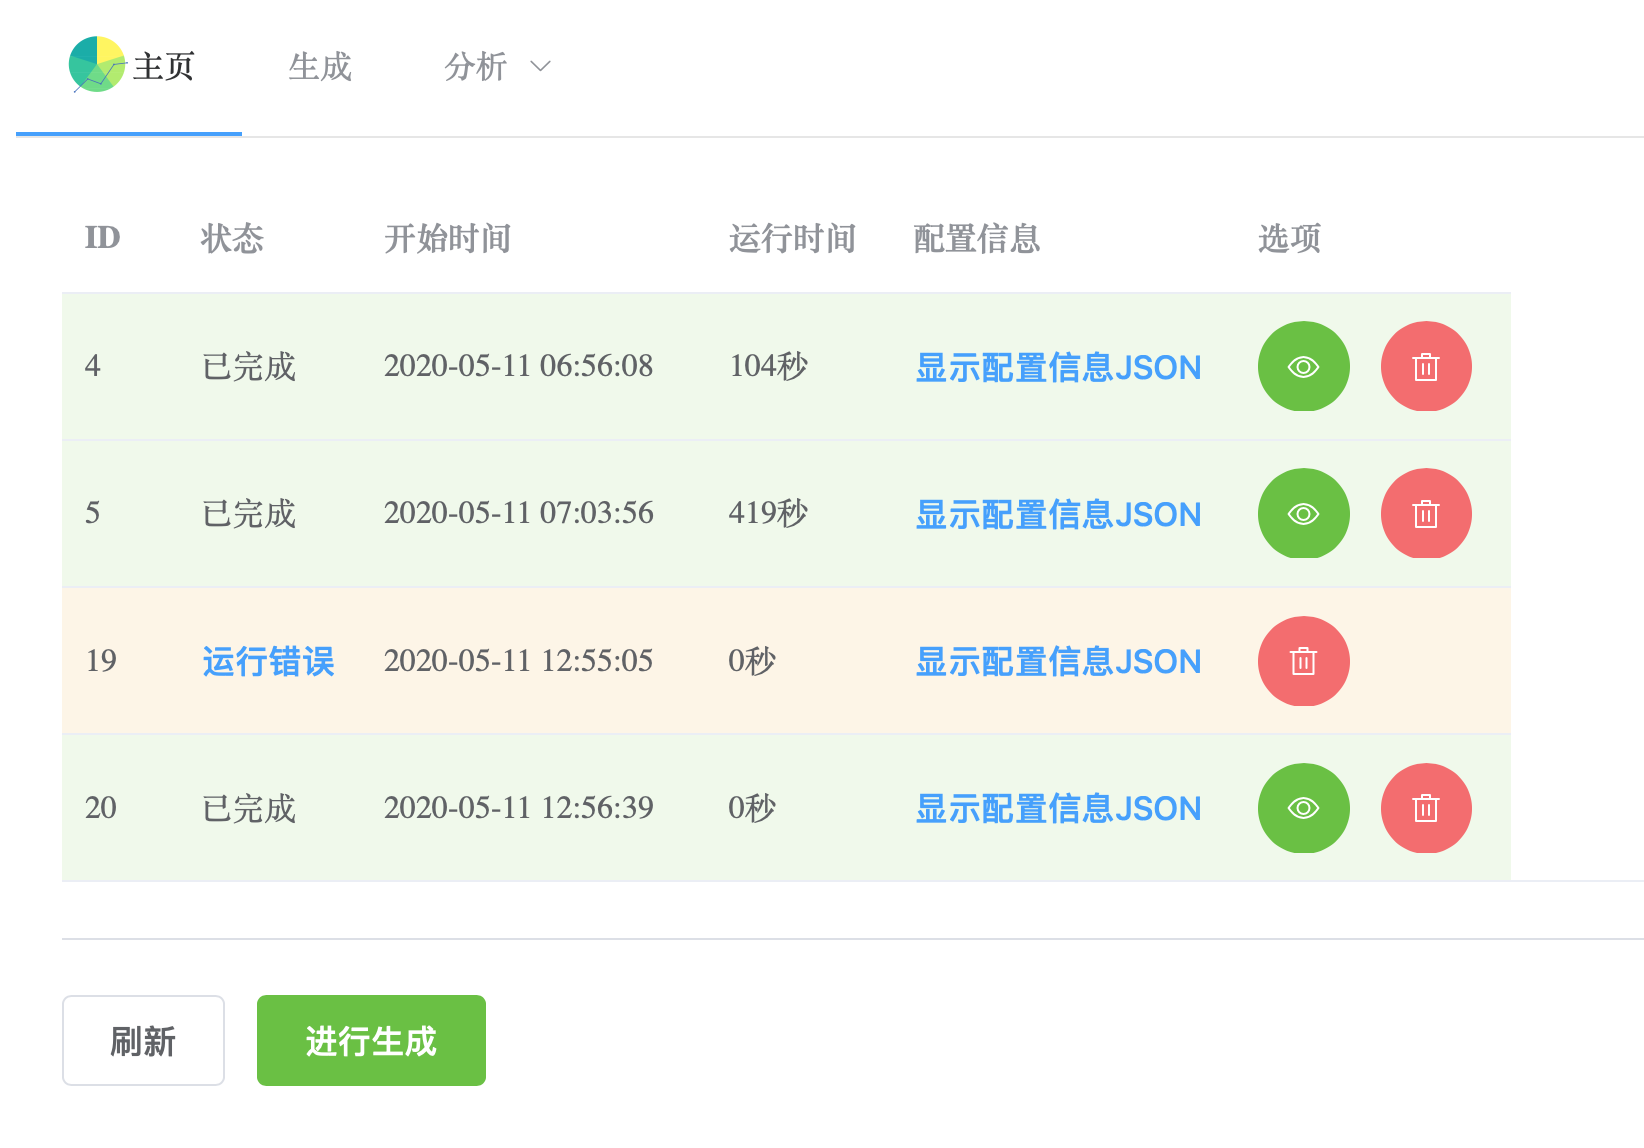
\includegraphics[scale=0.45]{frontend-home.png}
  \caption{管理系统-主页设计}
  \label{fig:frontend-home}
\end{figure}

在配置选择页面,用户可以用交互式操作进行每一个选项的详细配置。如图\ref{fig:iterations_node}、\ref{fig:edge_comm_event}所示。

\begin{figure}[H]
  \centering
  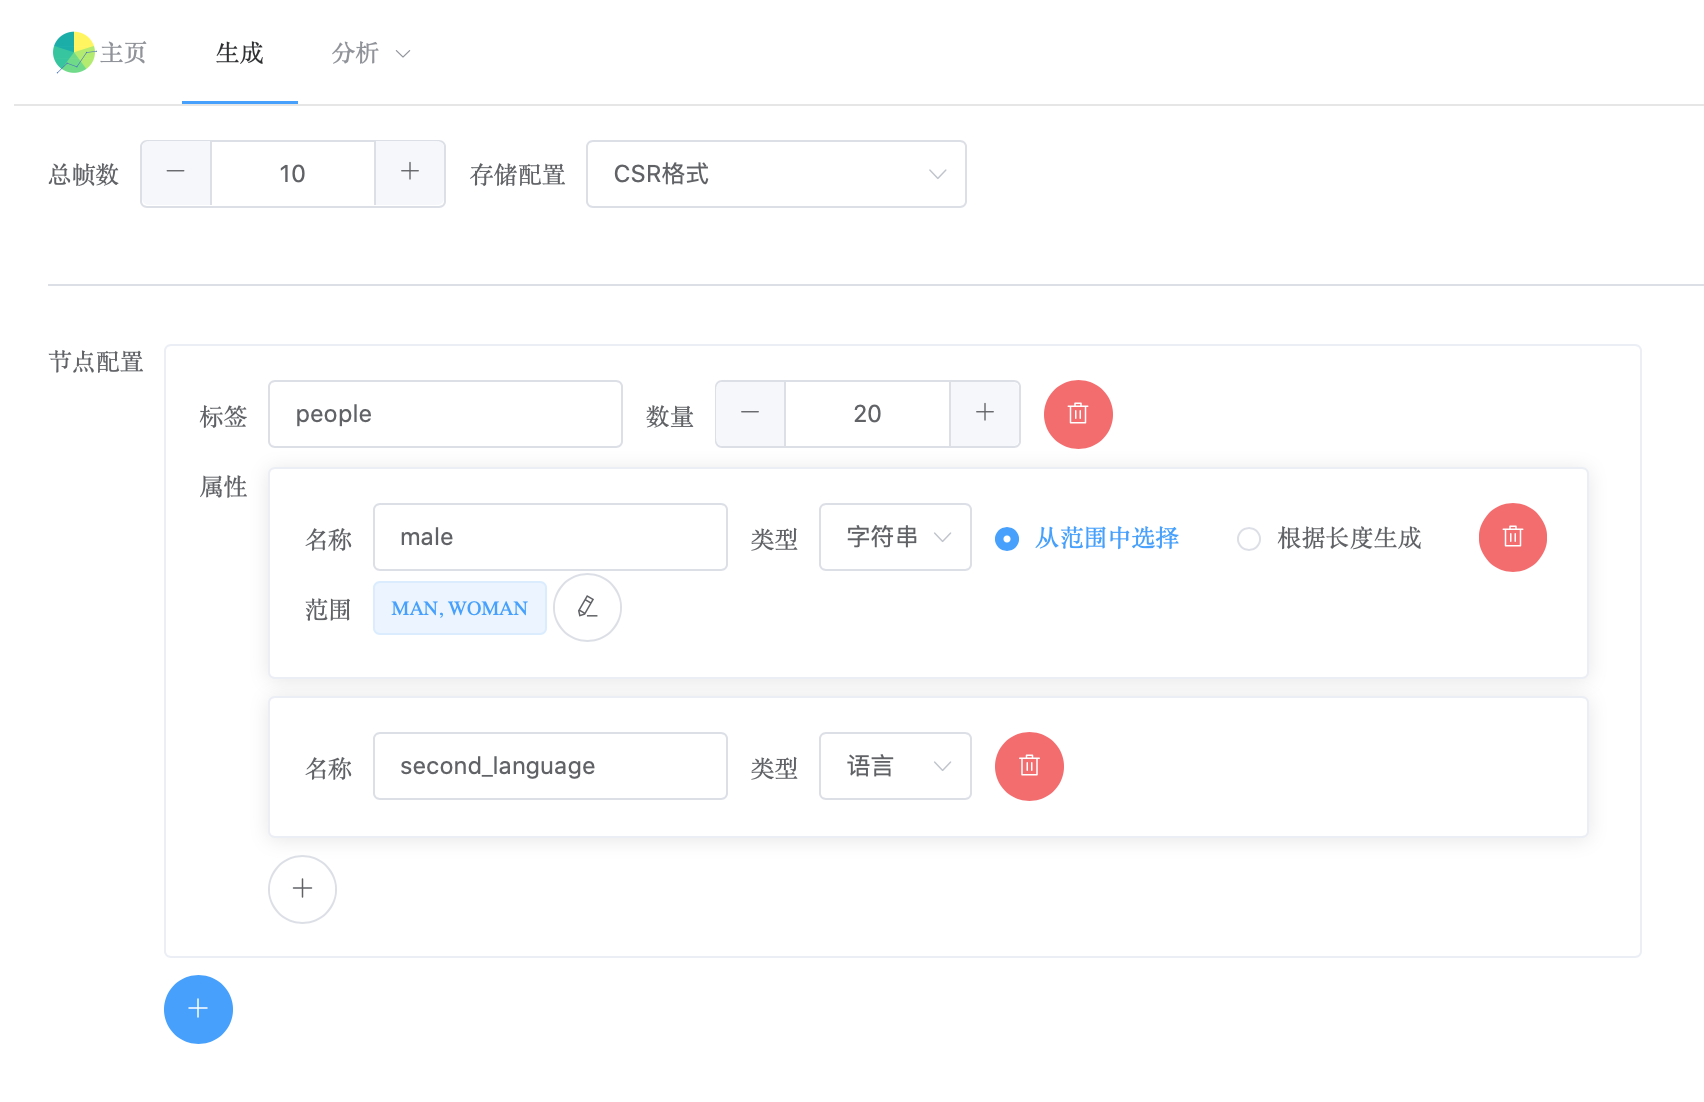
\includegraphics[scale=0.4]{iterations_node.png}
  \caption{管理系统-生成配置选项1}
  \label{fig:iterations_node}
\end{figure}

\begin{figure}[H]
  \centering
  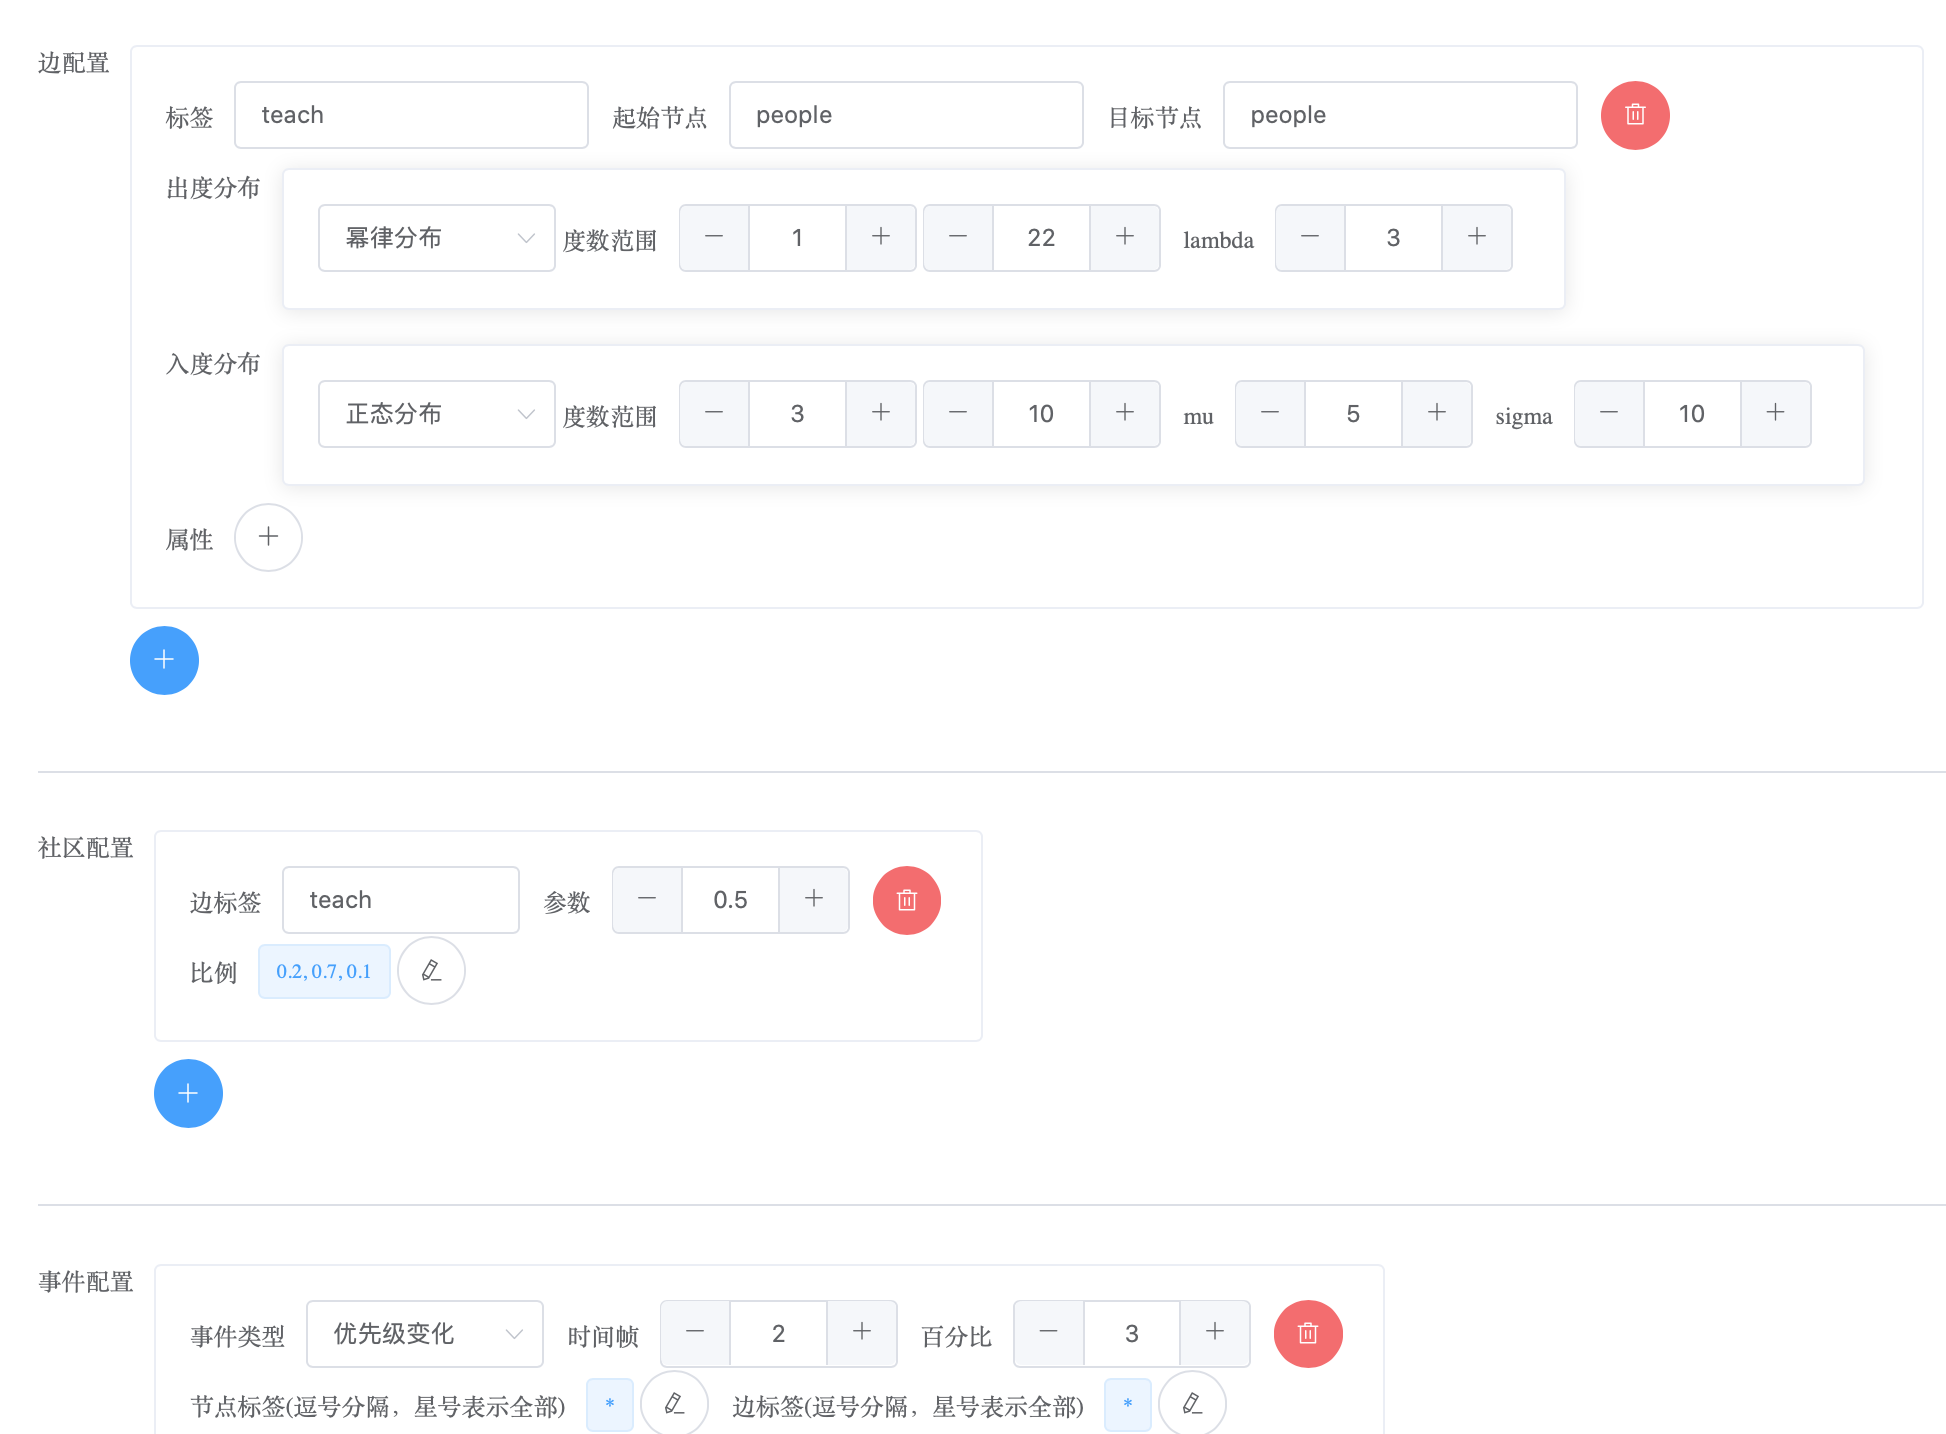
\includegraphics[scale=0.4]{edge_comm_event.png}
  \caption{管理系统-生成配置选项2}
  \label{fig:edge_comm_event}
\end{figure}

如图\ref{fig:analyzepage}所示,系统中实现了如下几种分析与可视化的显示:度数分布\footnote{度数分布部分展示每一个时刻对应的度数分布图}、度数变化\footnote{度数变化部分在选定一个节点,进行该节点度数变化分析}、节点变化\footnote{节点变化部分展示在各个事件中影响了哪些节点}、图可视化\footnote{图可视化部分会逐帧展示每一个时刻的图}。

\begin{figure}[H]
  \centering
  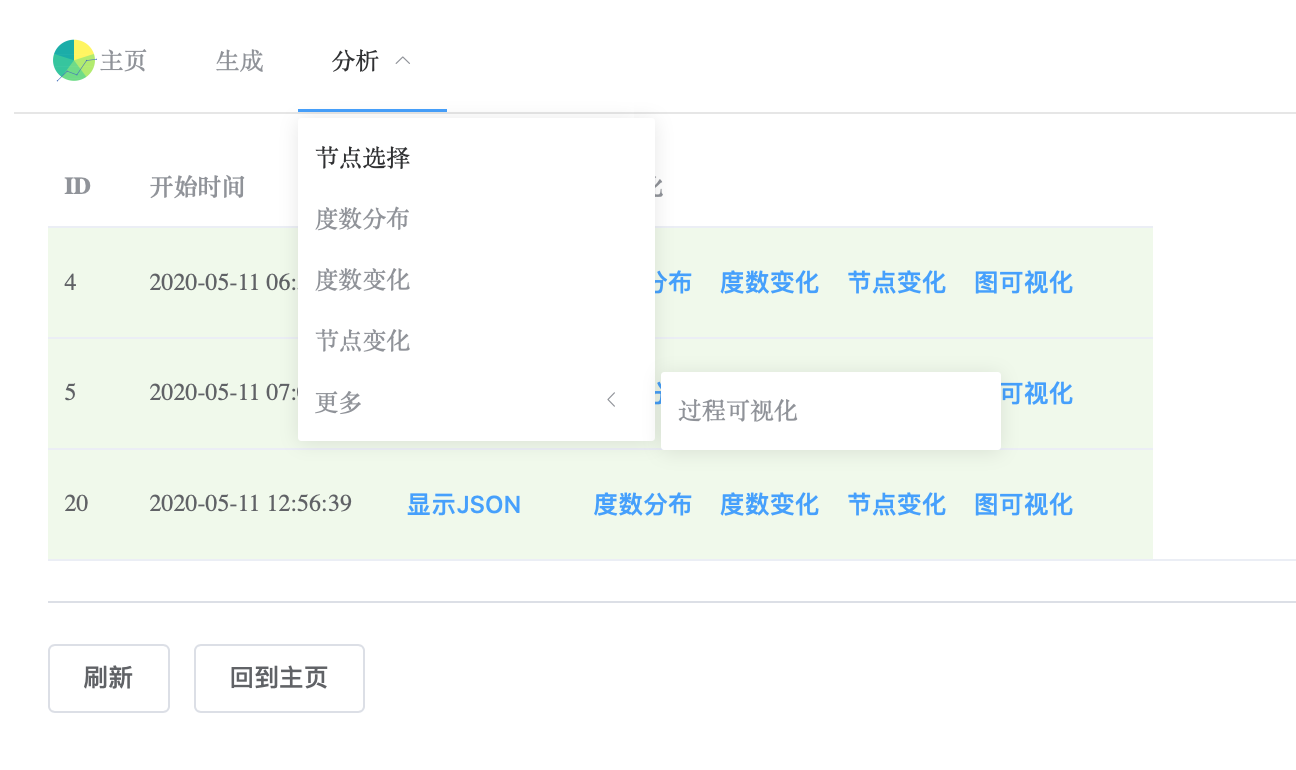
\includegraphics[scale=0.5]{analyzepage.png}
  \caption{管理系统-分析选项}
  \label{fig:analyzepage}
\end{figure}

以度数分布为例,其显示结果如图\ref{fig:degree_show}所示。选择边的标签、时刻信息、出度/入度分布之后,即可看到在这一个时刻的分布特征。

\begin{figure}[H]
  \centering
  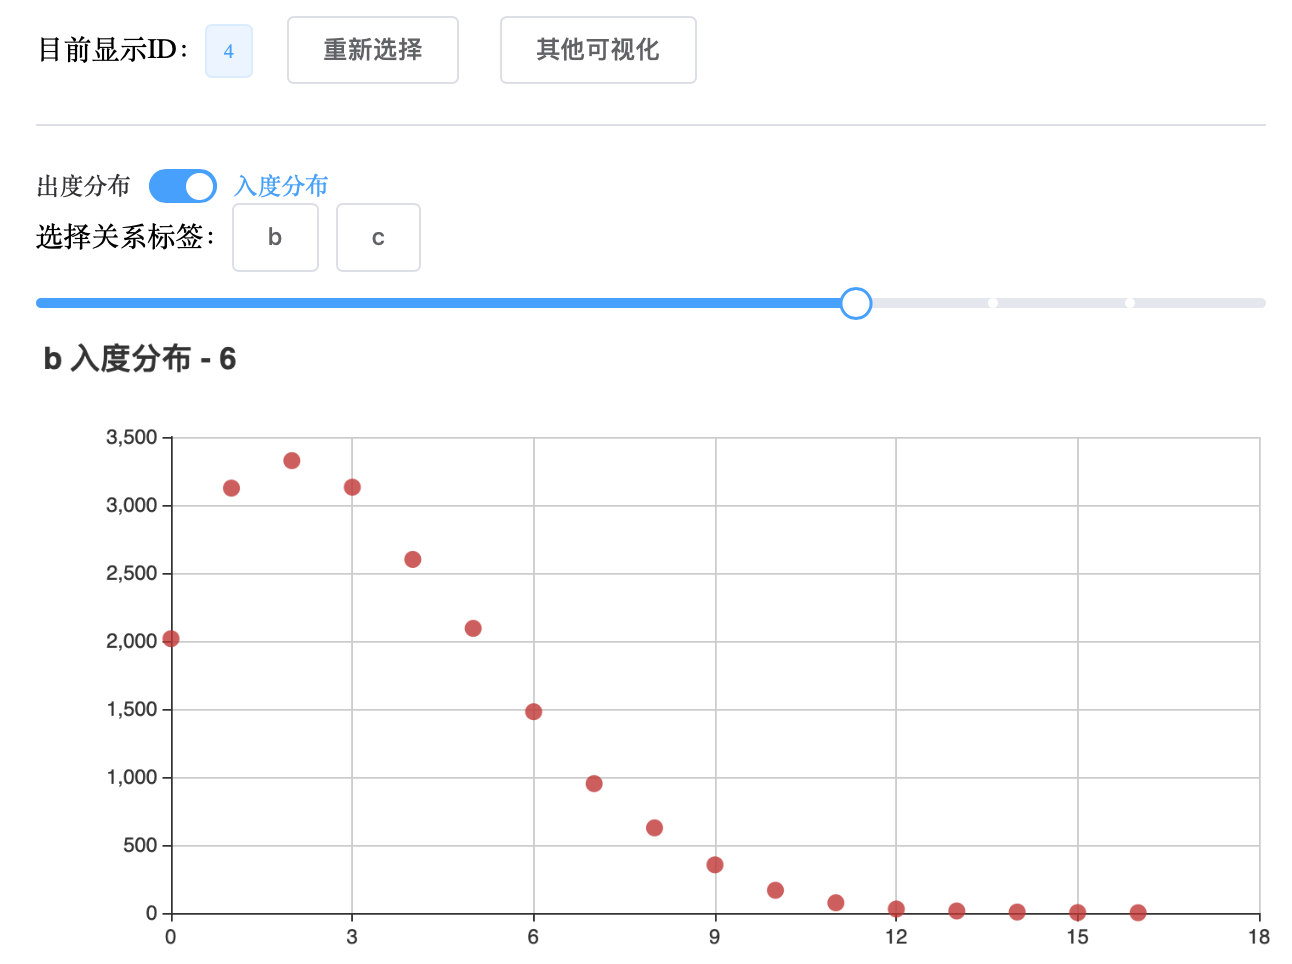
\includegraphics[scale=0.45]{degree_show.png}
  \caption{管理系统-度数分布分析}
  \label{fig:degree_show}
\end{figure}

\section{执行流程}

% 一个用户的典型操作过程与相应的前后端行为如下:

% \begin{enumerate}
%   \item 用户进入配置选择页面,进行所需动态图相关属性的配置(如图\ref{fig:iterations_node}、\ref{fig:edge_comm_event});
%   \item 前端将用户填写的配置信息转换为JSON格式,发送到后端;
%   \item 后端收到动态图生成请求与配置信息,分配一个新的线程进行生成操作,该线程会将生成任务相关信息存储到数据库中;
%   \item 用户获取生成结果,后端收到请求后在数据库中进行查询,若生成线程执行完成则将结果返回给前端进行结果的渲染与显示;
%   \item 用户选择进行可视化分析,后端收到请求后进行统计分析,将对应的结果返回前端进行渲染与展示。
% \end{enumerate}

% 具体执行流程如如图\ref{fig:stream}所示。

% \begin{figure}[H]
%   \centering
%   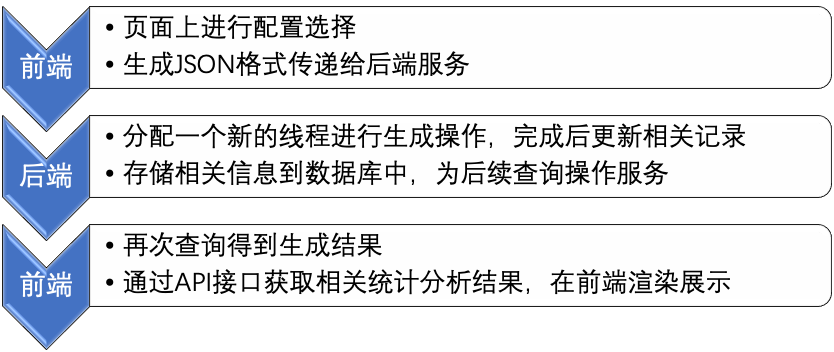
\includegraphics[scale=0.45]{stream.png}
%   \caption{管理系统-执行流程}
%   \label{fig:stream}
% \end{figure}

系统的具体执行流程如如图\ref{fig:uml_generate}与图\ref{fig:uml_analyze}所示。

\begin{figure}[H]
  \centering
  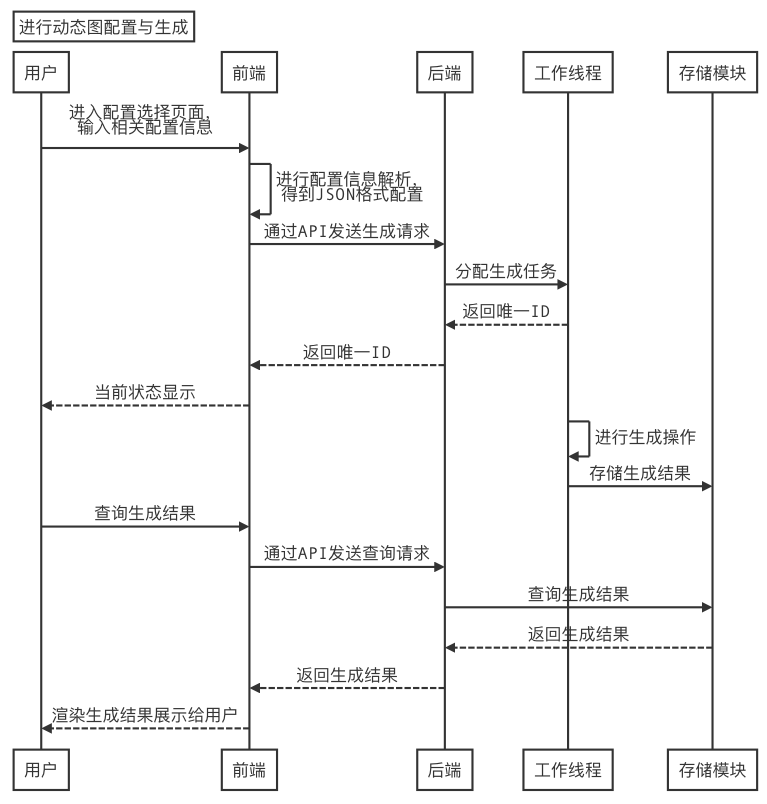
\includegraphics[scale=0.45]{uml_generate.png}
  \caption{动态图生成过程流程图}
  \label{fig:uml_generate}
\end{figure}

\begin{figure}[H]
  \centering
  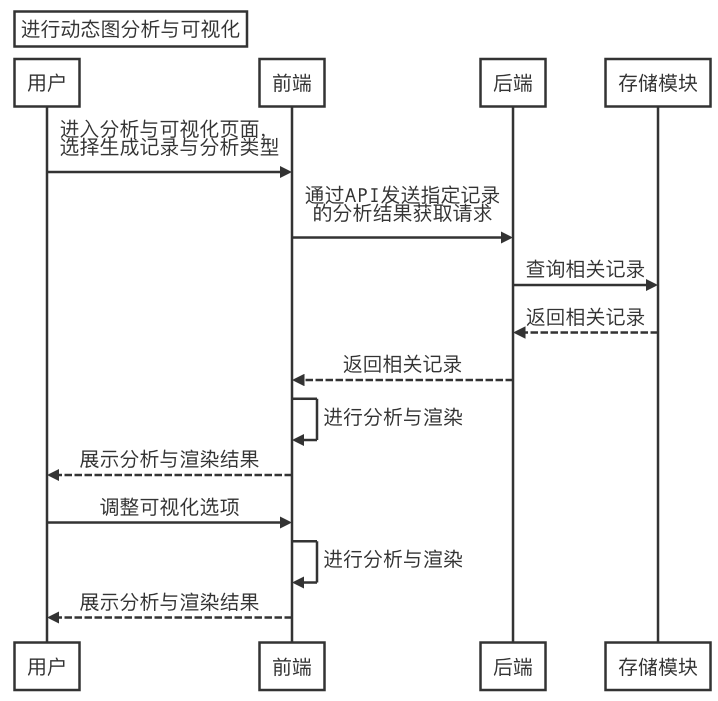
\includegraphics[scale=0.45]{uml_analyze.png}
  \caption{动态图分析与可视化流程图}
  \label{fig:uml_analyze}
\end{figure}